\documentclass[a4paper]{scrartcl}
\usepackage[utf8]{inputenc}
\usepackage[english]{babel}
\usepackage{graphicx}
\usepackage{lastpage}
\usepackage{pgf}
\usepackage{wrapfig}
\usepackage{fancyvrb}
\usepackage{fancyhdr}
\usepackage{hyperref}
\pagestyle{fancy}

\catcode`\_=\active
\protected\def_#1_{\textit{#1}}

% Create header and footer
\headheight 27pt
\pagestyle{fancyplain}
\lhead{\footnotesize{Network Programming, ID1212}}
\chead{\footnotesize{Project}}
\rhead{}
\lfoot{}
\cfoot{\thepage}
\rfoot{}

% Create title page
\title{Project - Distributed Rock-Paper-Scissors}
\subtitle{Network Programming, ID1212}
\author{Bernardo Gonzalez Riede, begr@kth.se}
\date{\today}

\begin{document}

\maketitle

%Introduction
\section{Introduction}
Goals:
\begin{itemize}
	\item Design, develop and deploy an Android app using the Android SDK
	\item Usage of the Android SDK and IDE tools
\end{itemize}


%Literature
\section{Literature Study}


%Literature
\section{Method}



\section{Result}

Link to public Github repository with code:
\href{https://github.com/MemBernd/ID1212-Android}{https://github.com/MemBernd/ID1212-Android}

\subsection{Layering}



%subsection covering implementation
\subsection{Communication}



\subsubsection{Possible communication errors no handled.}


\subsection{Distribution}



\subsection{Multiplayer}



%subsection covering gui
\subsection{GUI}

Figure \ref{fig:a1} shows the main activity when launched. 
The user is only taken to the gamestate server if he's able to successfully connect to the server.

\begin{figure}[h!]
  \begin{center}
    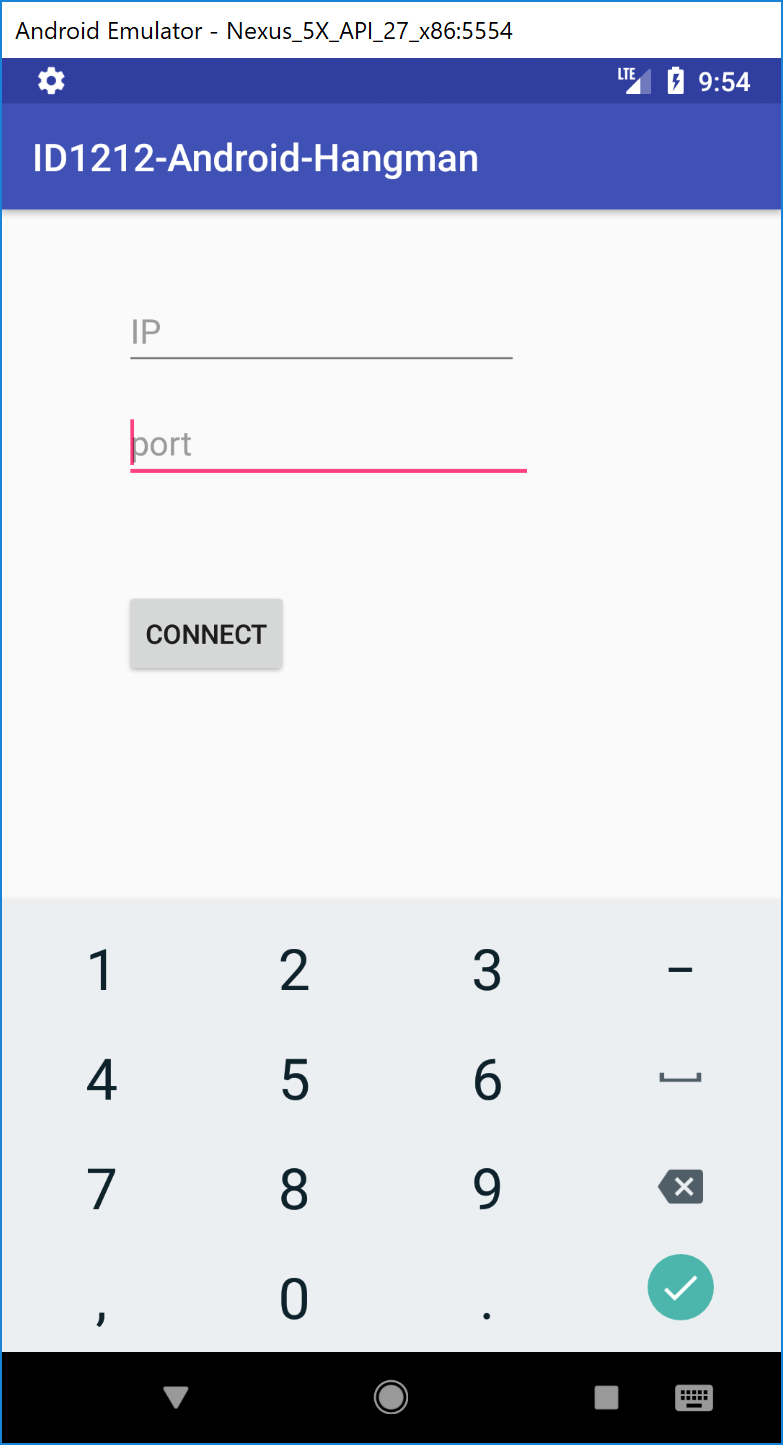
\includegraphics[scale=0.5]{Activity1.png}
    \caption{Initial interface}
    \label{fig:a1}
  \end{center}
\end{figure}


Figure \ref{fig:a2} is an example of a game after a game has been lost already.
In a second iteration it would be easily possible to extract the game score and attempts left counter and create a textview or similar to hold said information separately. Additionally, a afore mentioned toast can be seen at the bottom.

\begin{figure}[h!]
  \begin{center}
    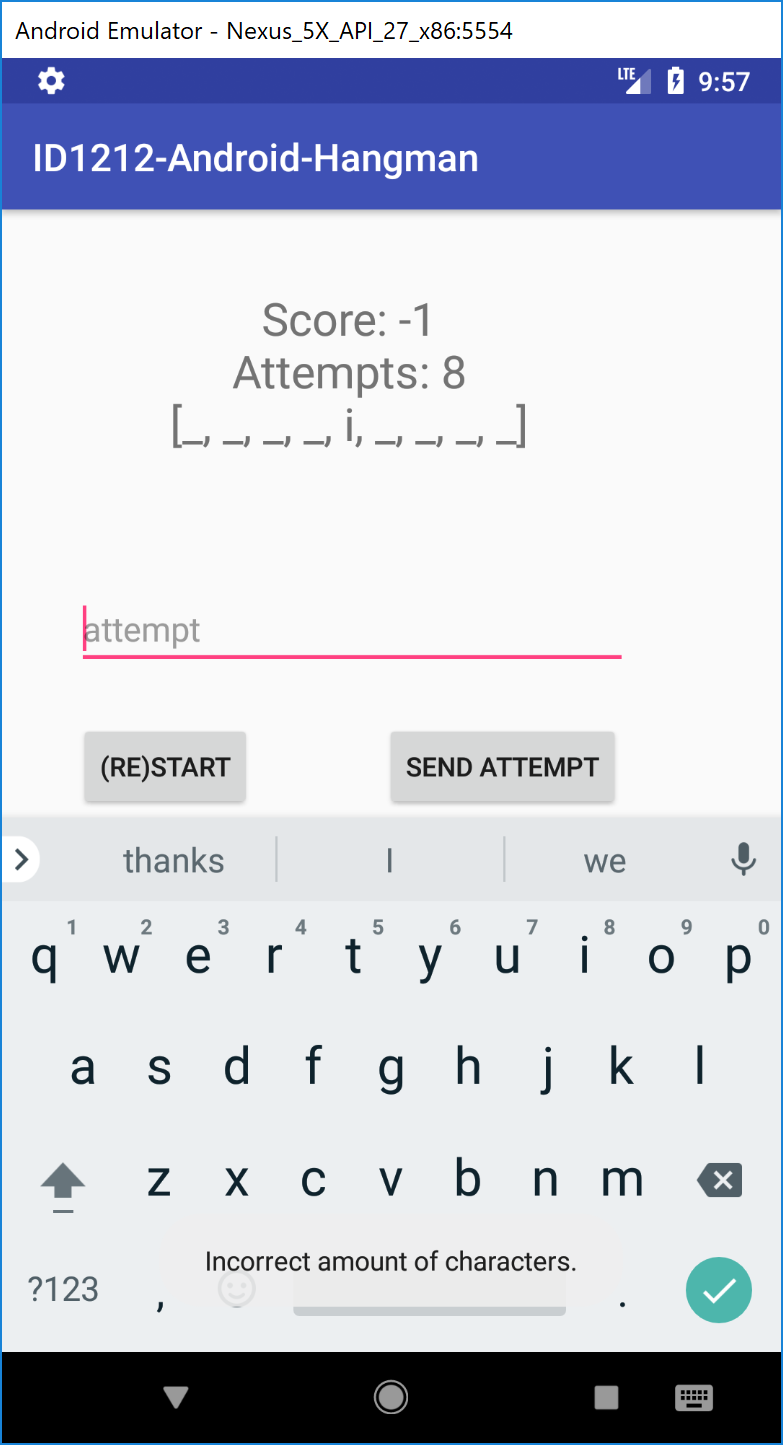
\includegraphics[scale=0.5]{Activity2.png}
    \caption{Game interface}
    \label{fig:a2}
  \end{center}
\end{figure}

%subsection discussion
\section{Discussion}


%subsection comments
\section{Comments About the Course}

It took around 15. 
\begin{itemize}
        \item 4 hours 20 min for coding.
        \item The report was written in one hour due to inadequate time management.
\end{itemize}




\end{document}
